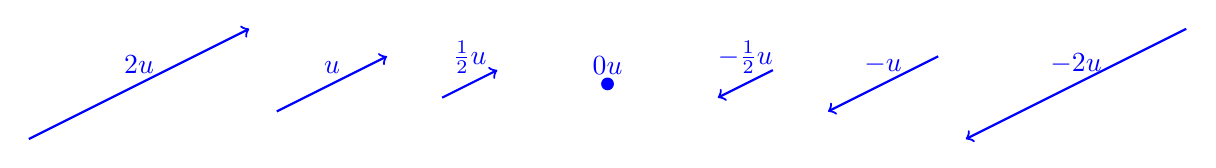
\begin{tikzpicture}[scale=0.7]
      \draw[->, thick, blue] (-10.5,-1)    -- node[above]{$2\vect{u}$} +(4,2);
      \draw[->, thick, blue] (-6,-0.5)  -- node[above]{$\vect{u}$} +(2,1);
      \draw[->, thick, blue] (-3,-0.25) -- node[above]{$\frac{1}{2}\vect{u}$} +(1,0.5);
      \draw[fill, blue](0,0) circle [radius=3pt] node[above]{$0\vect{u}$};
      \draw[->, thick, blue] (3,0.25)   -- node[above]{$-\frac{1}{2}\vect{u}$} +(-1,-0.5);
      \draw[->, thick, blue] (6,0.5)    -- node[above]{$-\vect{u}$} +(-2,-1);
      \draw[->, thick, blue] (10.5,1)      -- node[above]{$-2\vect{u}$} +(-4,-2);
    \end{tikzpicture}
